\section{First closed loop}
\subsection{simulink diagram}

\subsection{simulink}
\begin{figure}[H]
	\centering
	\begin{subfigure}[b]{0.45\textwidth}
		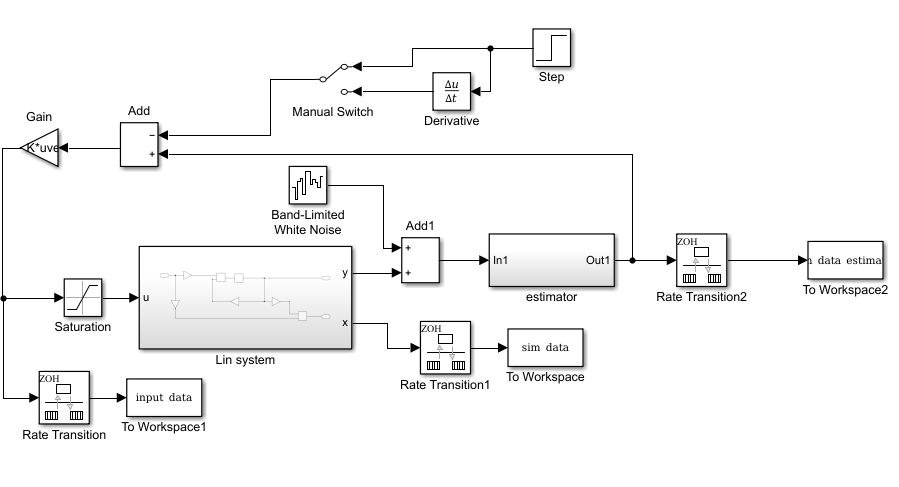
\includegraphics[width=\textwidth]{./part2_LQR1/not_generated/simulink_main.png}
		\caption{}
		\label{fig:main simulink part3 LQR}
	\end{subfigure}
	\begin{subfigure}[b]{0.45\textwidth}
		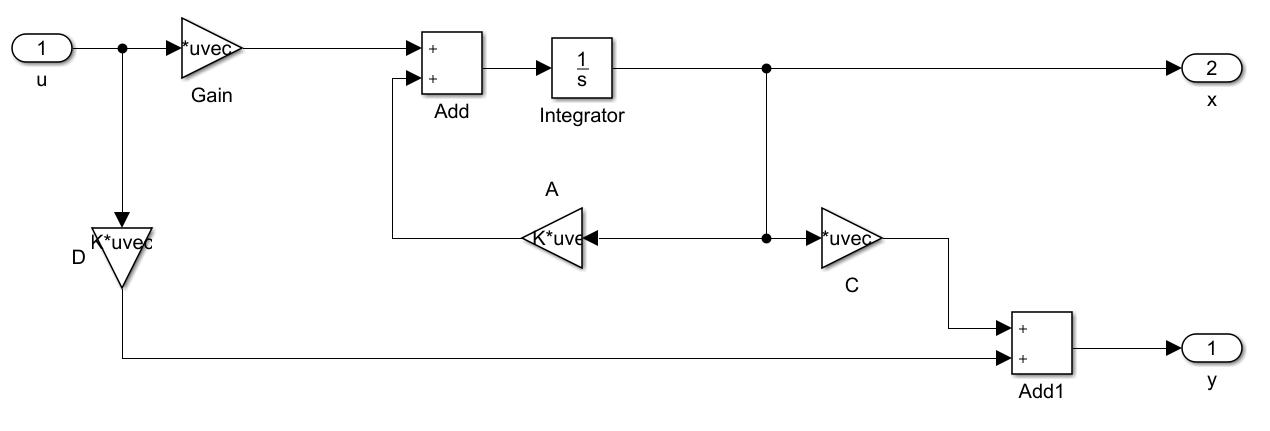
\includegraphics[width=\textwidth]{./part3_LQR2/not_generated/simulink_lin_sys.png}
		\caption{linear system}
	\end{subfigure}
	\caption{}
\end{figure}

\subsection{Determine the values of Q and R}
With default Q and R
$$
Q=\begin{bmatrix}
4 & 0 & 0 & 0 \\
0 & 20 & 0 & 0 \\
0 & 0 & 0 & 0 \\
0 & 0 & 0 & 0 \\
\end{bmatrix}
R=1.5
$$
\begin{figure}[H]
	\centering
	\begin{subfigure}[b]{0.45\textwidth}
		\includegraphics[width=\textwidth]{./part2_LQR1/1_default_QR_states.png}
		\caption{plot of the states in function of time}
	\end{subfigure}
	\begin{subfigure}[b]{0.45\textwidth}
		\includegraphics[width=\textwidth]{./part2_LQR1/1_default_QR_inputs.png}
		\caption{plot of the signal send to the motor in function of time}
	\end{subfigure}
	\caption{RIP with default values for Q and R}
	\label{fig:default}
\end{figure}

After evaluating a step response we think that the system can react faster because the limits of the motor aren't reached yet. Therefore we lower $ R = 0.5$. In figure \ref{fig:lowR} you can see that the response is faster and the input-voltage of the motor is higher.

\begin{figure}[H]
	\centering
	\begin{subfigure}[b]{0.45\textwidth}
		\includegraphics[width=\textwidth]{./part2_LQR1/2_lower_R_states.png}
		\caption{plot of the states in function of time}
	\end{subfigure}
	\begin{subfigure}[b]{0.45\textwidth}
		\includegraphics[width=\textwidth]{./part2_LQR1/2_lower_R_inputs.png}
		\caption{plot of the signal send to the motor in function of time}
	\end{subfigure}
	\caption{RIP lower R}
	\label{fig:lowR}
\end{figure}

When we see the step response we think that by adding some weight to $\theta$ that the system becomes still a bit faster. So by changing the weight of $\theta$ from 4 to 10 the step response becomes indeed faster. The effect can be seen in figure \ref{fig:heighT}.

\begin{figure}[H]
	\centering
	\begin{subfigure}[b]{0.45\textwidth}
		\includegraphics[width=\textwidth]{./part2_LQR1/3_increase_theta_states.png}
		\caption{plot of the states in function of time}
	\end{subfigure}
	\begin{subfigure}[b]{0.45\textwidth}
		\includegraphics[width=\textwidth]{./part2_LQR1/3_increase_theta_inputs.png}
		\caption{plot of the signal send to the motor in function of time}
	\end{subfigure}
	\caption{RIP increase $\theta$}
	\label{fig:heighT}
\end{figure}

For increasing the stability we now increase the weight of $\alpha$ from 20 to 60. The effect on the speed is minimal.

\begin{figure}[H]
	\centering
	\begin{subfigure}[b]{0.45\textwidth}
		\includegraphics[width=\textwidth]{./part2_LQR1/4_increase_alpha_states.png}
		\caption{plot of the states in function of time}
	\end{subfigure}
	\begin{subfigure}[b]{0.45\textwidth}
		\includegraphics[width=\textwidth]{./part2_LQR1/4_increase_alpha_inputs.png}
		\caption{plot of the signal send to the motor in function of time}
	\end{subfigure}
	\caption{RIP increase $\alpha$}
\end{figure}

Because we don't like zeros on the diagonal of the weighting matrix we changed from the beginning the angular velocity weights to 0.1. As last step we've set the weight of $\dot{\alpha}$ to 1. The final values for Q and R are:
$$
Q=\begin{bmatrix}
10 & 0 & 0 & 0 \\
0 & 60 & 0 & 0 \\
0 & 0 & 0 & 0 \\
0 & 0 & 0 & 1 \\
\end{bmatrix}
R=0.5
$$

\begin{figure}[H]
	\centering
	\begin{subfigure}[b]{0.45\textwidth}
		\includegraphics[width=\textwidth]{./part2_LQR1/5_increase_alpha_dot_states.png}
		\caption{plot of the states in function of time}
	\end{subfigure}
	\begin{subfigure}[b]{0.45\textwidth}
		\includegraphics[width=\textwidth]{./part2_LQR1/5_increase_alpha_dot_inputs.png}
		\caption{plot of the signal send to the motor in function of time}
	\end{subfigure}
	\caption{RIP increase $\dot{\alpha}$}
\end{figure}

%\begin{figure}[H]
%	\centering
%	\begin{subfigure}[b]{0.45\textwidth}
%		\includegraphics[width=\textwidth]{./part2_LQR1/final_states.png}
%		\caption{plot of the states in function of time}
%	\end{subfigure}
%	\begin{subfigure}[b]{0.45\textwidth}
%		\includegraphics[width=\textwidth]{./part2_LQR1/final_inputs.png}
%		\caption{plot of the signal send to the motor in function of time}
%	\end{subfigure}
%	\caption{RIP final states}
%\end{figure}



\subsection{simulated setpoint change: TODO}